% % \subsection{Kiến trúc hệ thống}
% % \lipsum[1]

\subsection{Kiến trúc hệ thống}
\lipsum[1]


\subsubsection{Quản lý các thông tin bí mật (doppler)}

Quản lý các thông tin bí mật là một phần cực kỳ quan trọng. Đặc biệt khi hệ thống được thiết kế theo kiến trúc microservices.
Khi dự án có nhiều service, việc sử dụng file .env độc lập cho từng service sẽ gây khó khăn trong việc quản lý, cấu hình, đồng bộ và bảo mật.


\begin{block}{Ứng dụng trong đồ án}
Trong đồ án này, em sử dụng Doppler
– một nền tảng quản lý thông tin bí mật tập trung.
Việc áp dụng Doppler mang lại một không gian lưu trữ an toàn,
thống nhất (Single Source of Truth) cho toàn bộ hệ thống.


\end{block}


\begin{figure}[H]
\centering
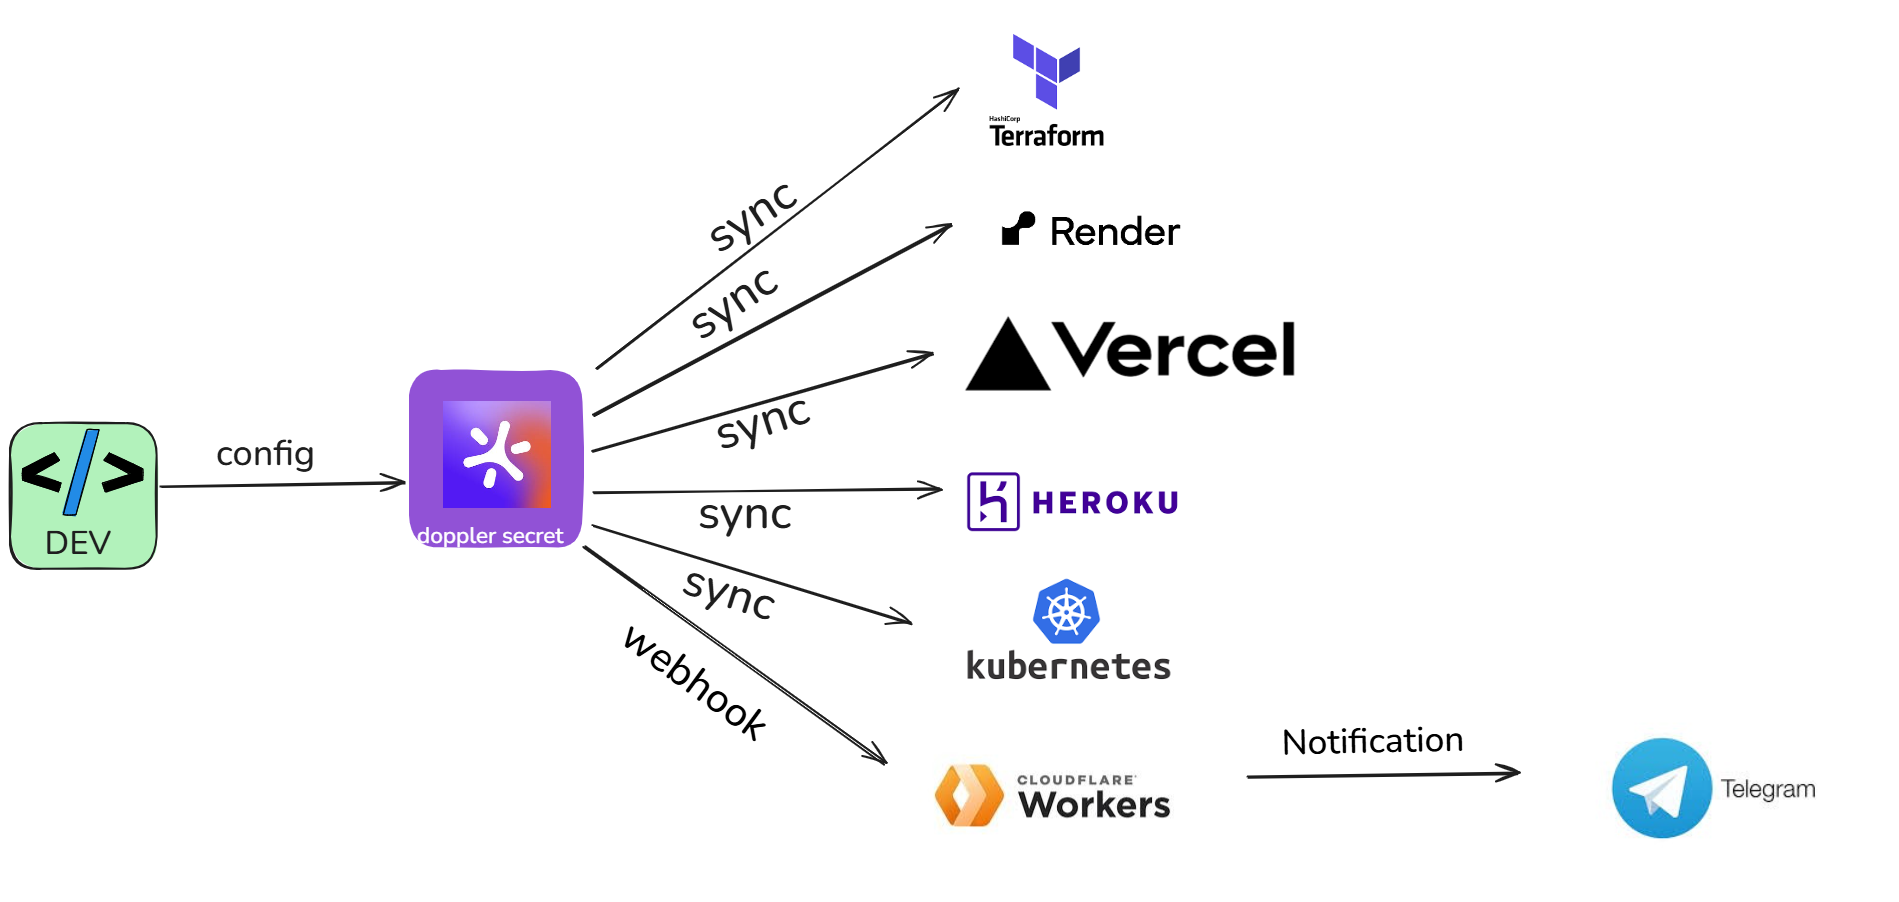
\includegraphics[scale = 0.2]{pictures/secret-by-doppler.excalidraw.png}
\caption{Sơ đồ quản lý secret bằng doppler}
\end{figure}


Cấu hình chia nhỏ bí mật theo từng nhu cầu sử dụng trong doppler


\begin{figure}[H]
\centering
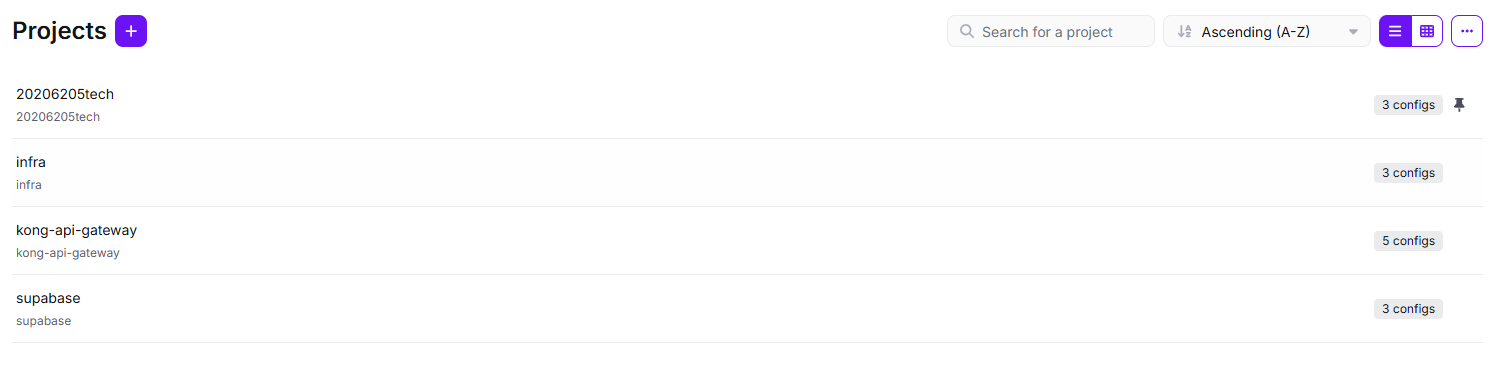
\includegraphics[scale = 0.4]{pictures/doppler-projects.png}
\caption{Cấu hình chia nhỏ bí mật theo từng nhu cầu sử dụng trong doppler}
\end{figure}


\begin{figure}[H]
\centering
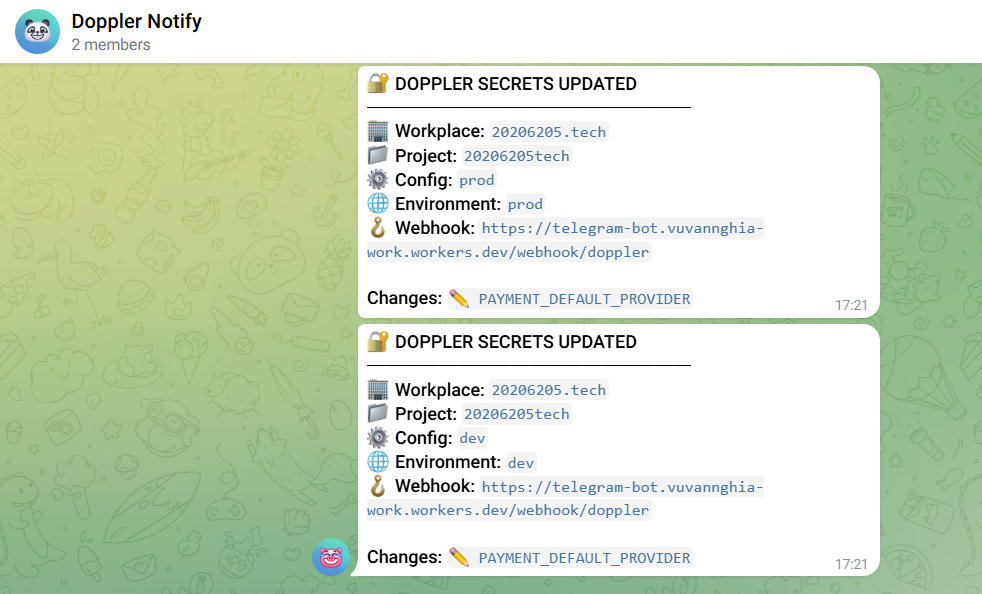
\includegraphics[scale = 0.4]{pictures/doppler-telegram2.png}
\caption{Cấu hình chia nhỏ bí mật theo từng nhu cầu sử dụng trong doppler}
\end{figure}


\subsubsection{CI/CD (Github Action)}


CI/CD là
phương pháp tự động hóa
quy trình tích hợp
và triển khai phần mềm.
Phương pháp này giúp
đẩy nhanh tốc độ, giảm thiểu lỗi thủ công
và duy trì độ ổn định cho hệ thống.
GitHub Actions là công cụ CI/CD mạnh mẽ được tích hợp sẵn trên GitHub.


\begin{figure}[H]
\centering
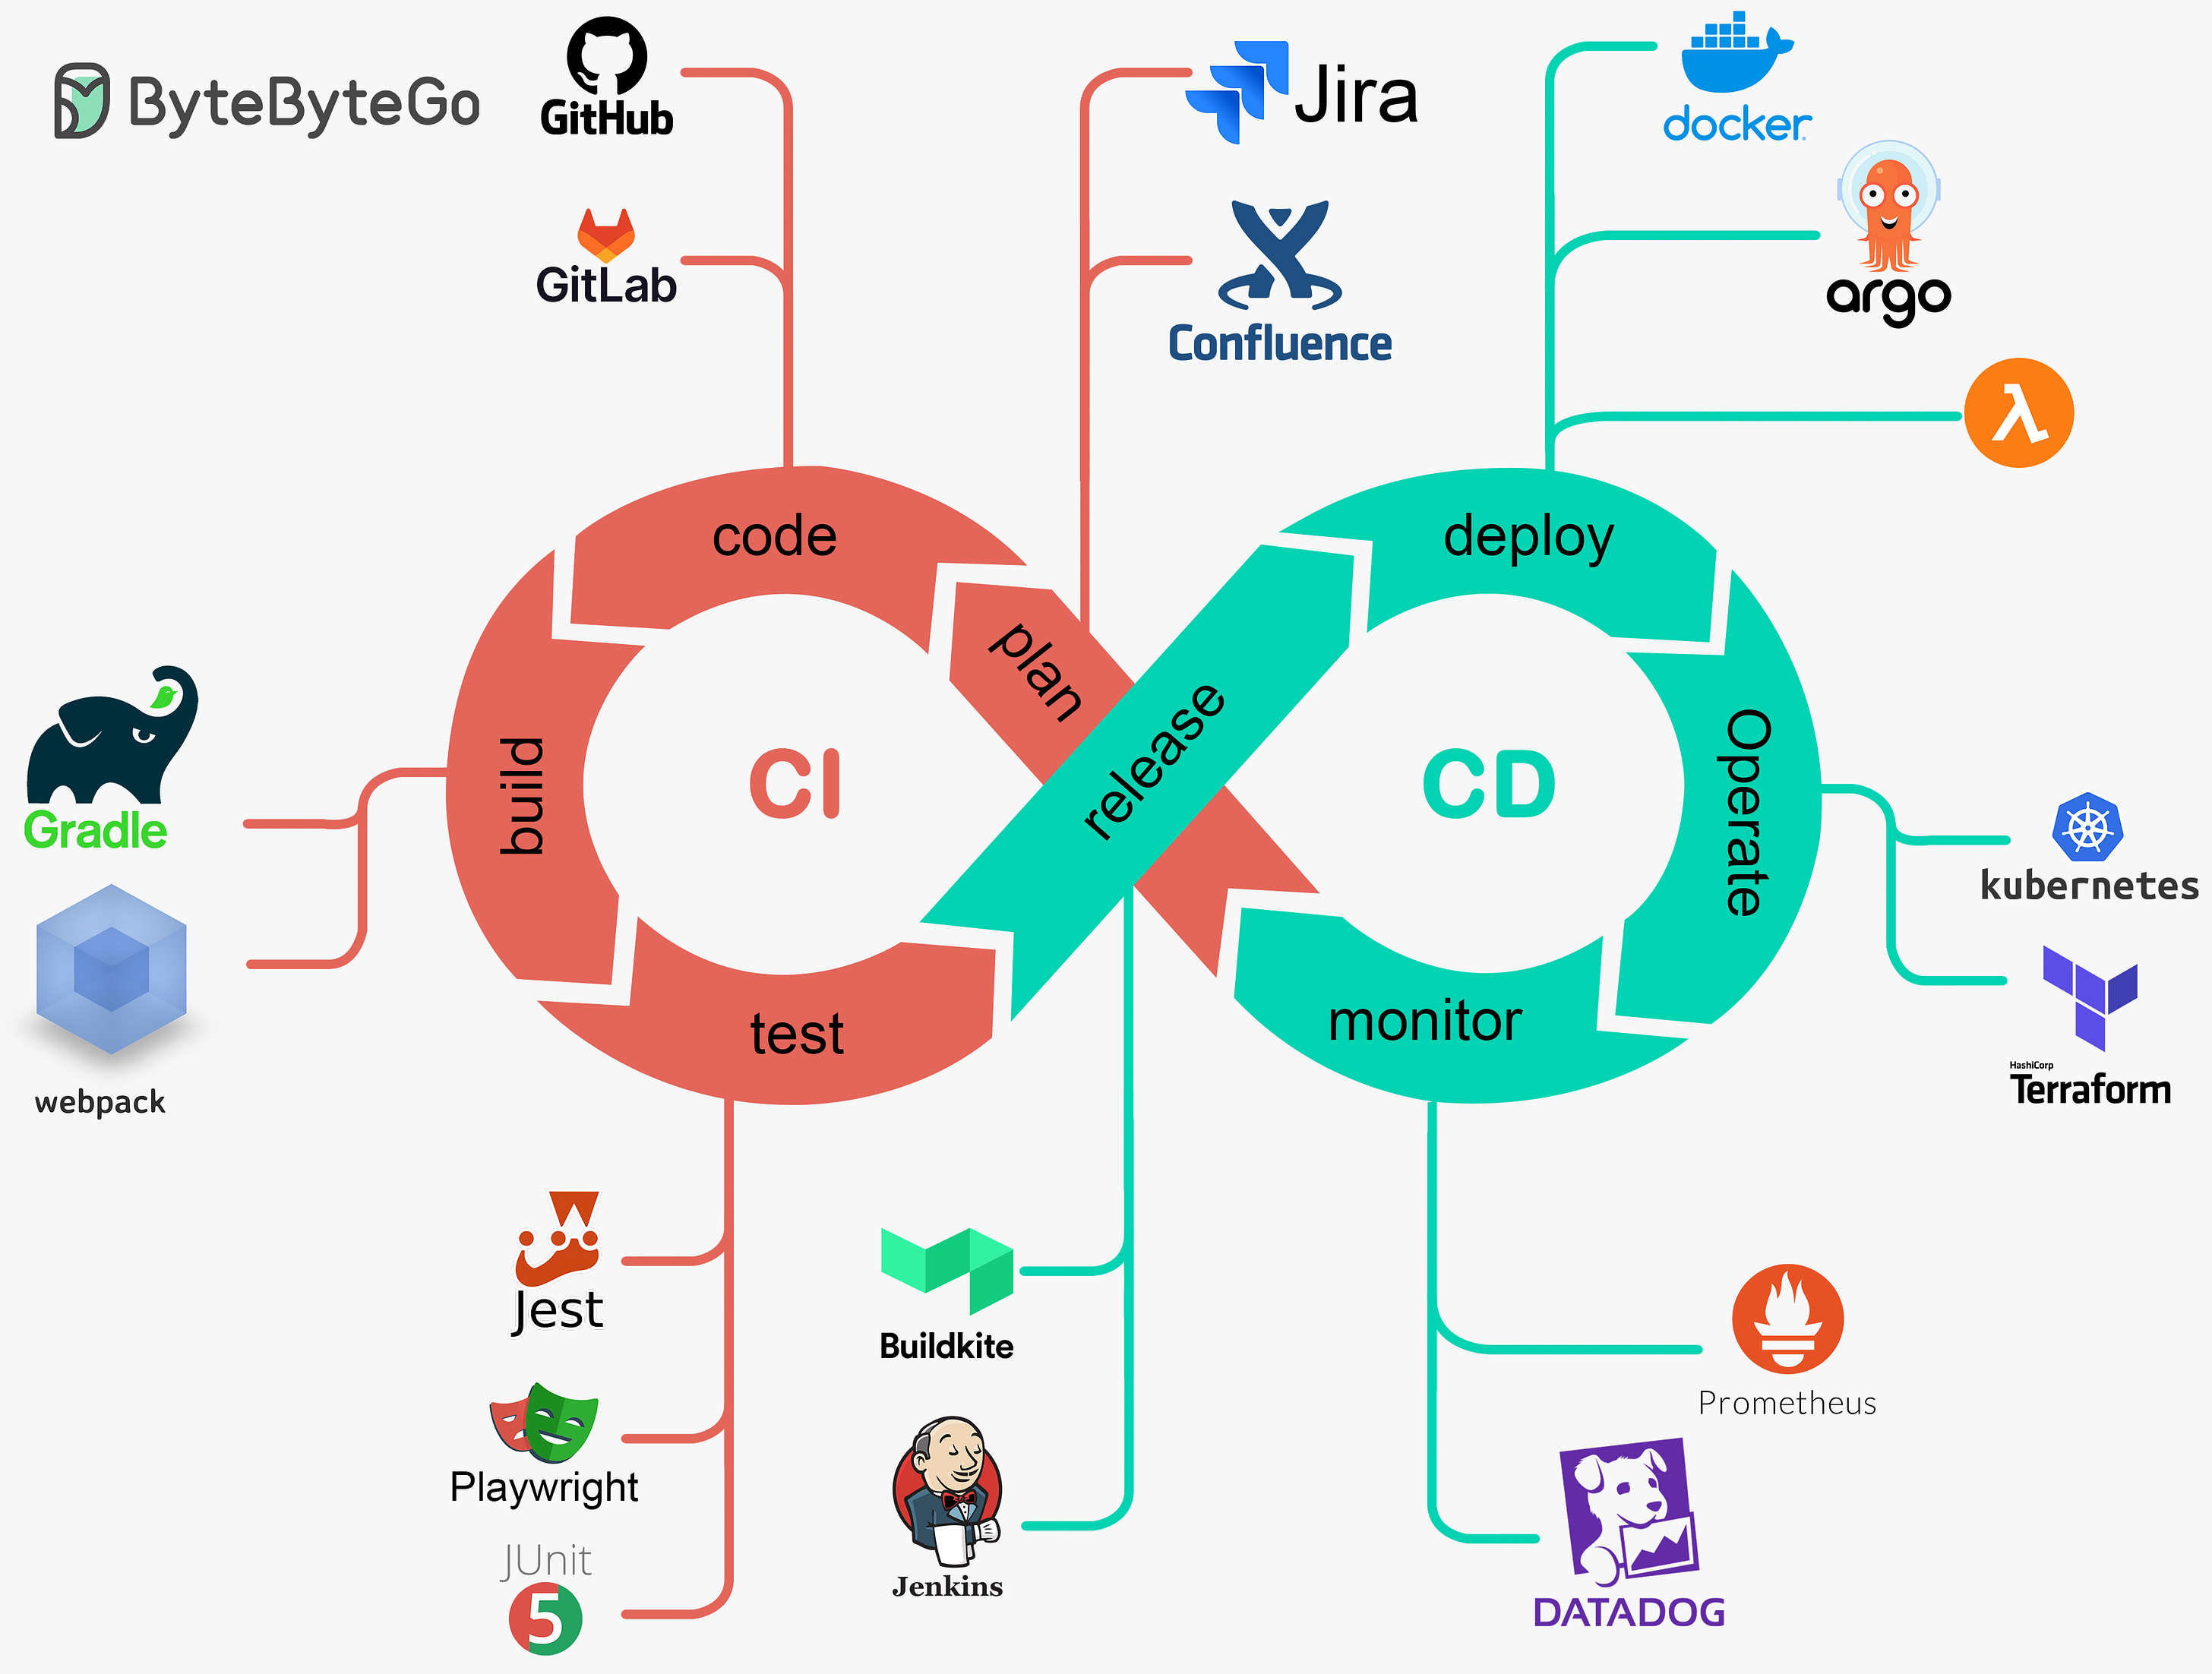
\includegraphics[scale = 0.1]{pictures/cicd-overview.jpg}
\caption{Cấu hình chia nhỏ bí mật theo từng nhu cầu sử dụng trong doppler}
\end{figure}


Sơ đồ CI/CD bằng Github Action


\begin{figure}[H]
\centering
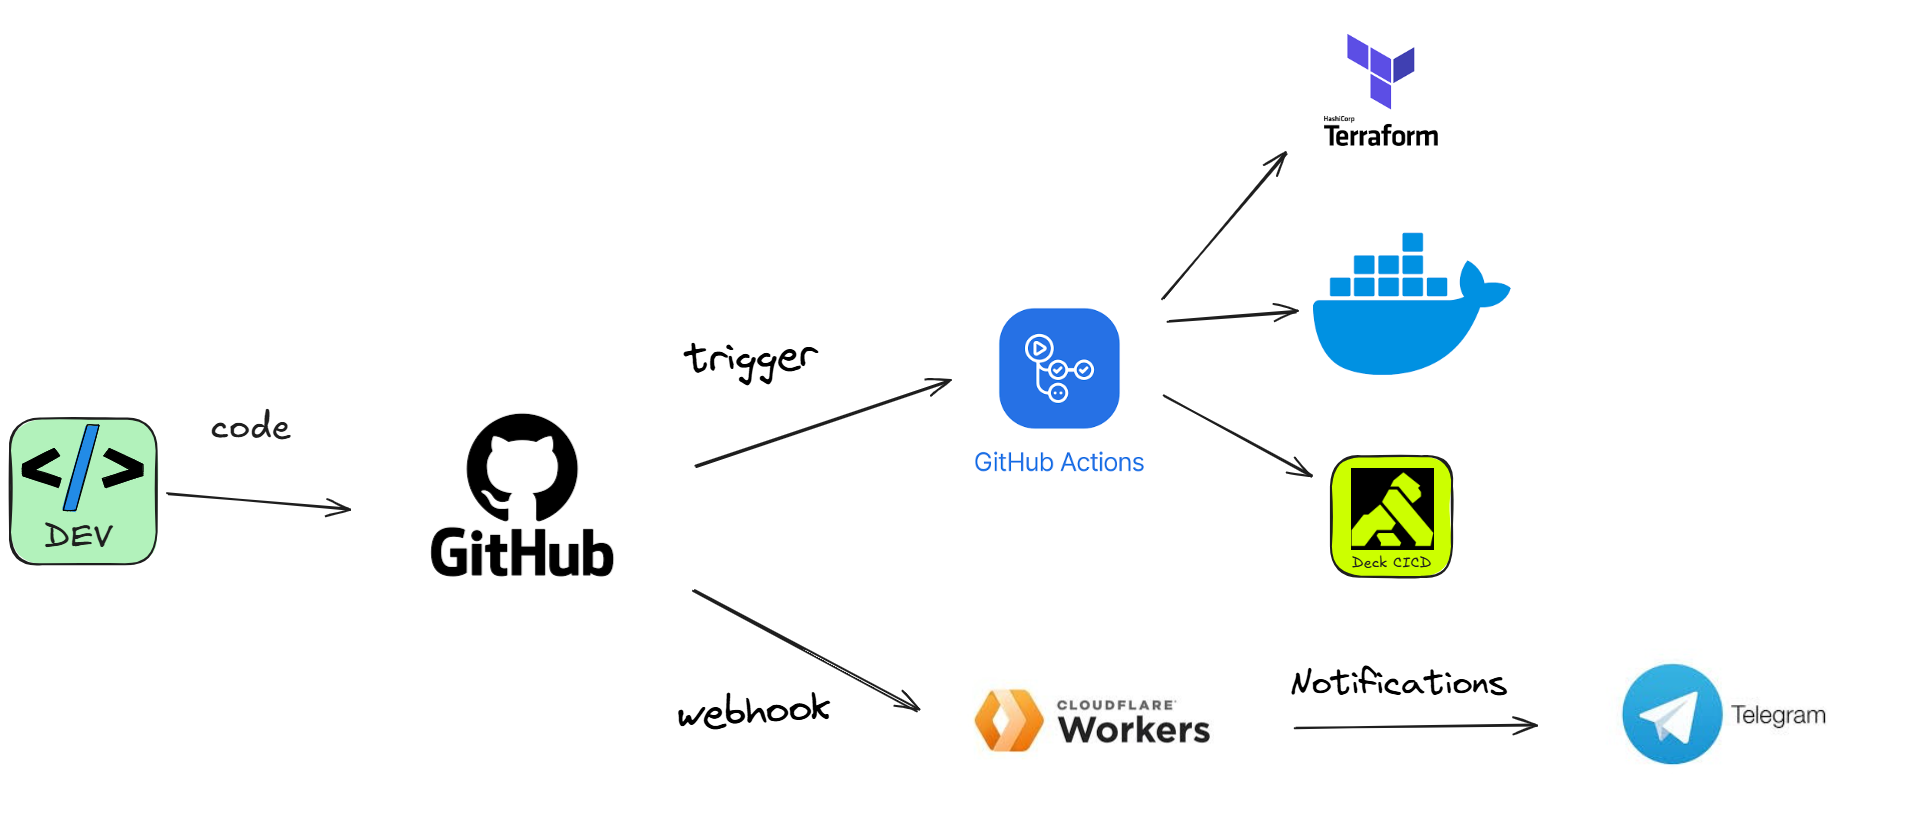
\includegraphics[scale = 0.2]{pictures/cicd-by-github-action.excalidraw.png}
\caption{Cấu hình chia nhỏ bí mật theo từng nhu cầu sử dụng trong doppler}
\end{figure}


\begin{block}{Ứng dụng trong đồ án}


Trong đồ án này,
hệ thống vừa sử dụng Github Action miễn phí của Github,
vừa sử dụng Self-hosted runner trên VPS.


\end{block}


\subsubsection{Cơ sở hạ tầng dưới dạng mã (terraform)}


\begin{figure}[H]
\centering
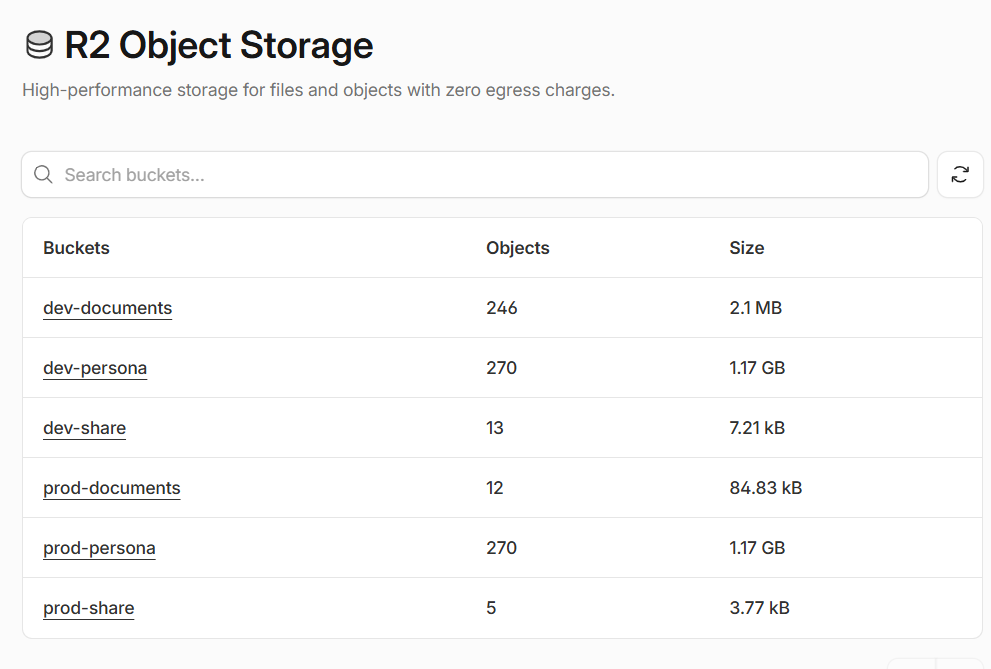
\includegraphics[scale = 0.2]{pictures/cloudflare-R2.png}
\caption{Cấu hình chia nhỏ bí mật theo từng nhu cầu sử dụng trong doppler}
\end{figure}


Trong công nghệ phần mềm việc cấu hình các cơ sở hạ tầng thủ công có thể gây sai sót, mất nhiều thời gian hoặc khi muốn tạo lại chính xác rất khó và khi cần xóa thì cũng sẽ phải ấn thủ công dẫn đến thiếu sót, gây rủi ro. Việc sử dụng Infrastructure as Code (IaC) sẽ khắc phục được vấn đề đó.


\begin{block}{Ứng dụng trong đồ án}


Trong đồ án này,
em sử dụng Terraform
để quản lý cấu hình một số hạ tầng của các nhà cung cấp
có hỗ trợ terraform giúp định nghĩa
và quản lý hạ tầng của dự án một cách tự động thay
vì thao tác thủ công.


\end{block}


\begin{itemize}

\item langsmith: theo dõi RAG
\item oracle: tạo vps
\item cloudflare: cấu hình DNS, bucket R2 file, tunnel
\item aiven: kafka
\item supabase: auth google
\item Neon: database postgres VBPL=>
\item digitalocean xxxxxxxxxxxxxx: database postgres VBPL
\item heroku: payment service
\end{itemize}


Kết quả kafka trong aiven được tạo tự động từ terraform


\begin{figure}[H]
\centering
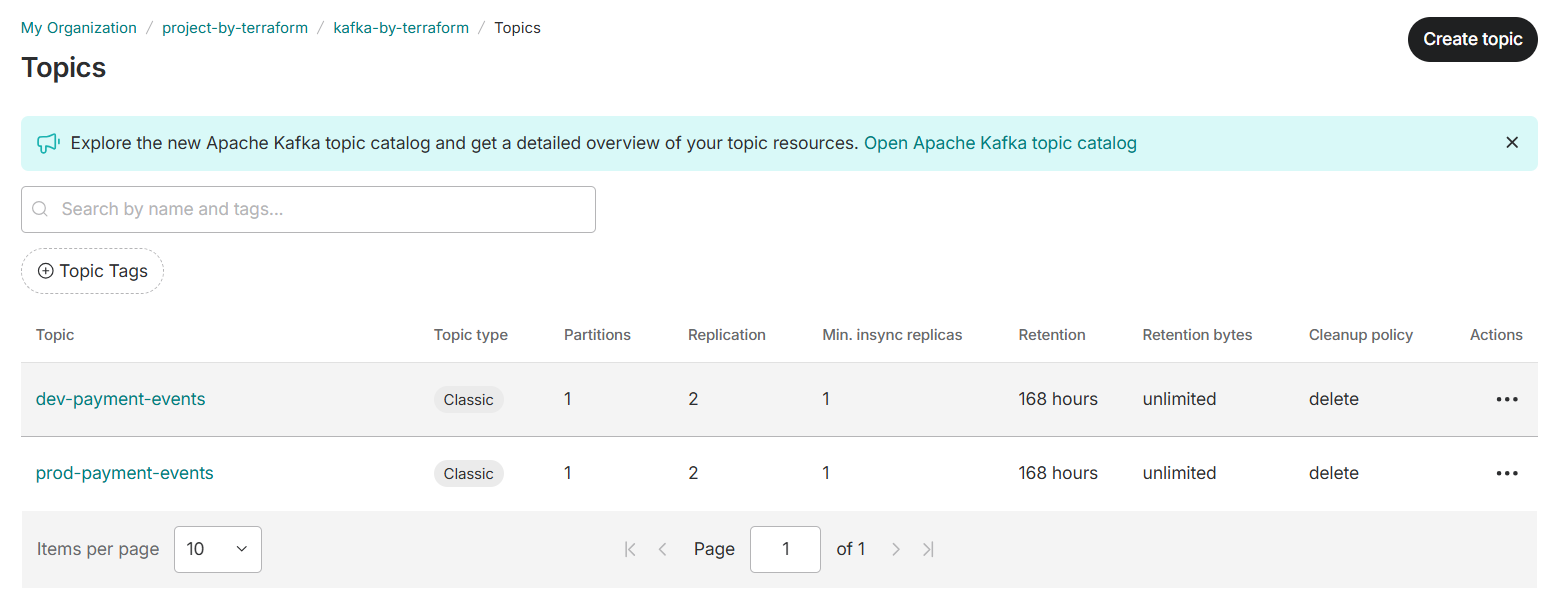
\includegraphics[scale = 0.2]{pictures/kafka-aiven-terraform.png}
\caption{Cấu hình chia nhỏ bí mật theo từng nhu cầu sử dụng trong doppler}
\end{figure}


\begin{figure}[H]
\centering
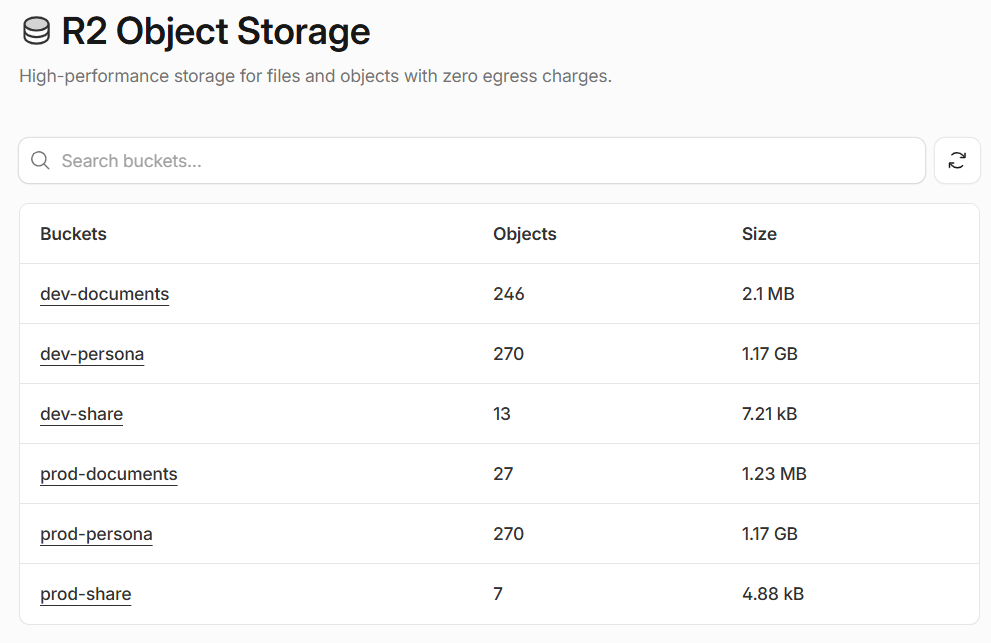
\includegraphics[scale = 0.2]{pictures/cloudflare-r2-terraform.png}
\caption{Cấu hình chia nhỏ bí mật theo từng nhu cầu sử dụng trong doppler}
\end{figure}


% TODO: tttt NEON tạo hẳn project cho riêng, độc lập, tránh giới hạn
% neon-limit-free.png


\begin{figure}[H]
\centering
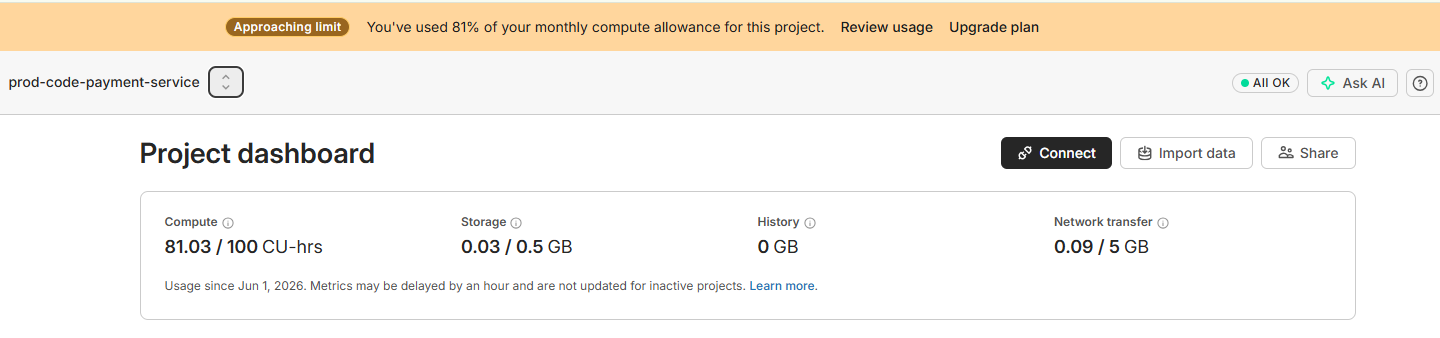
\includegraphics[scale = 0.2]{pictures/neon-limit-free.png}
\caption{Cấu hình chia nhỏ bí mật theo từng nhu cầu sử dụng trong doppler}
\end{figure}
\begin{figure}[H]
\centering
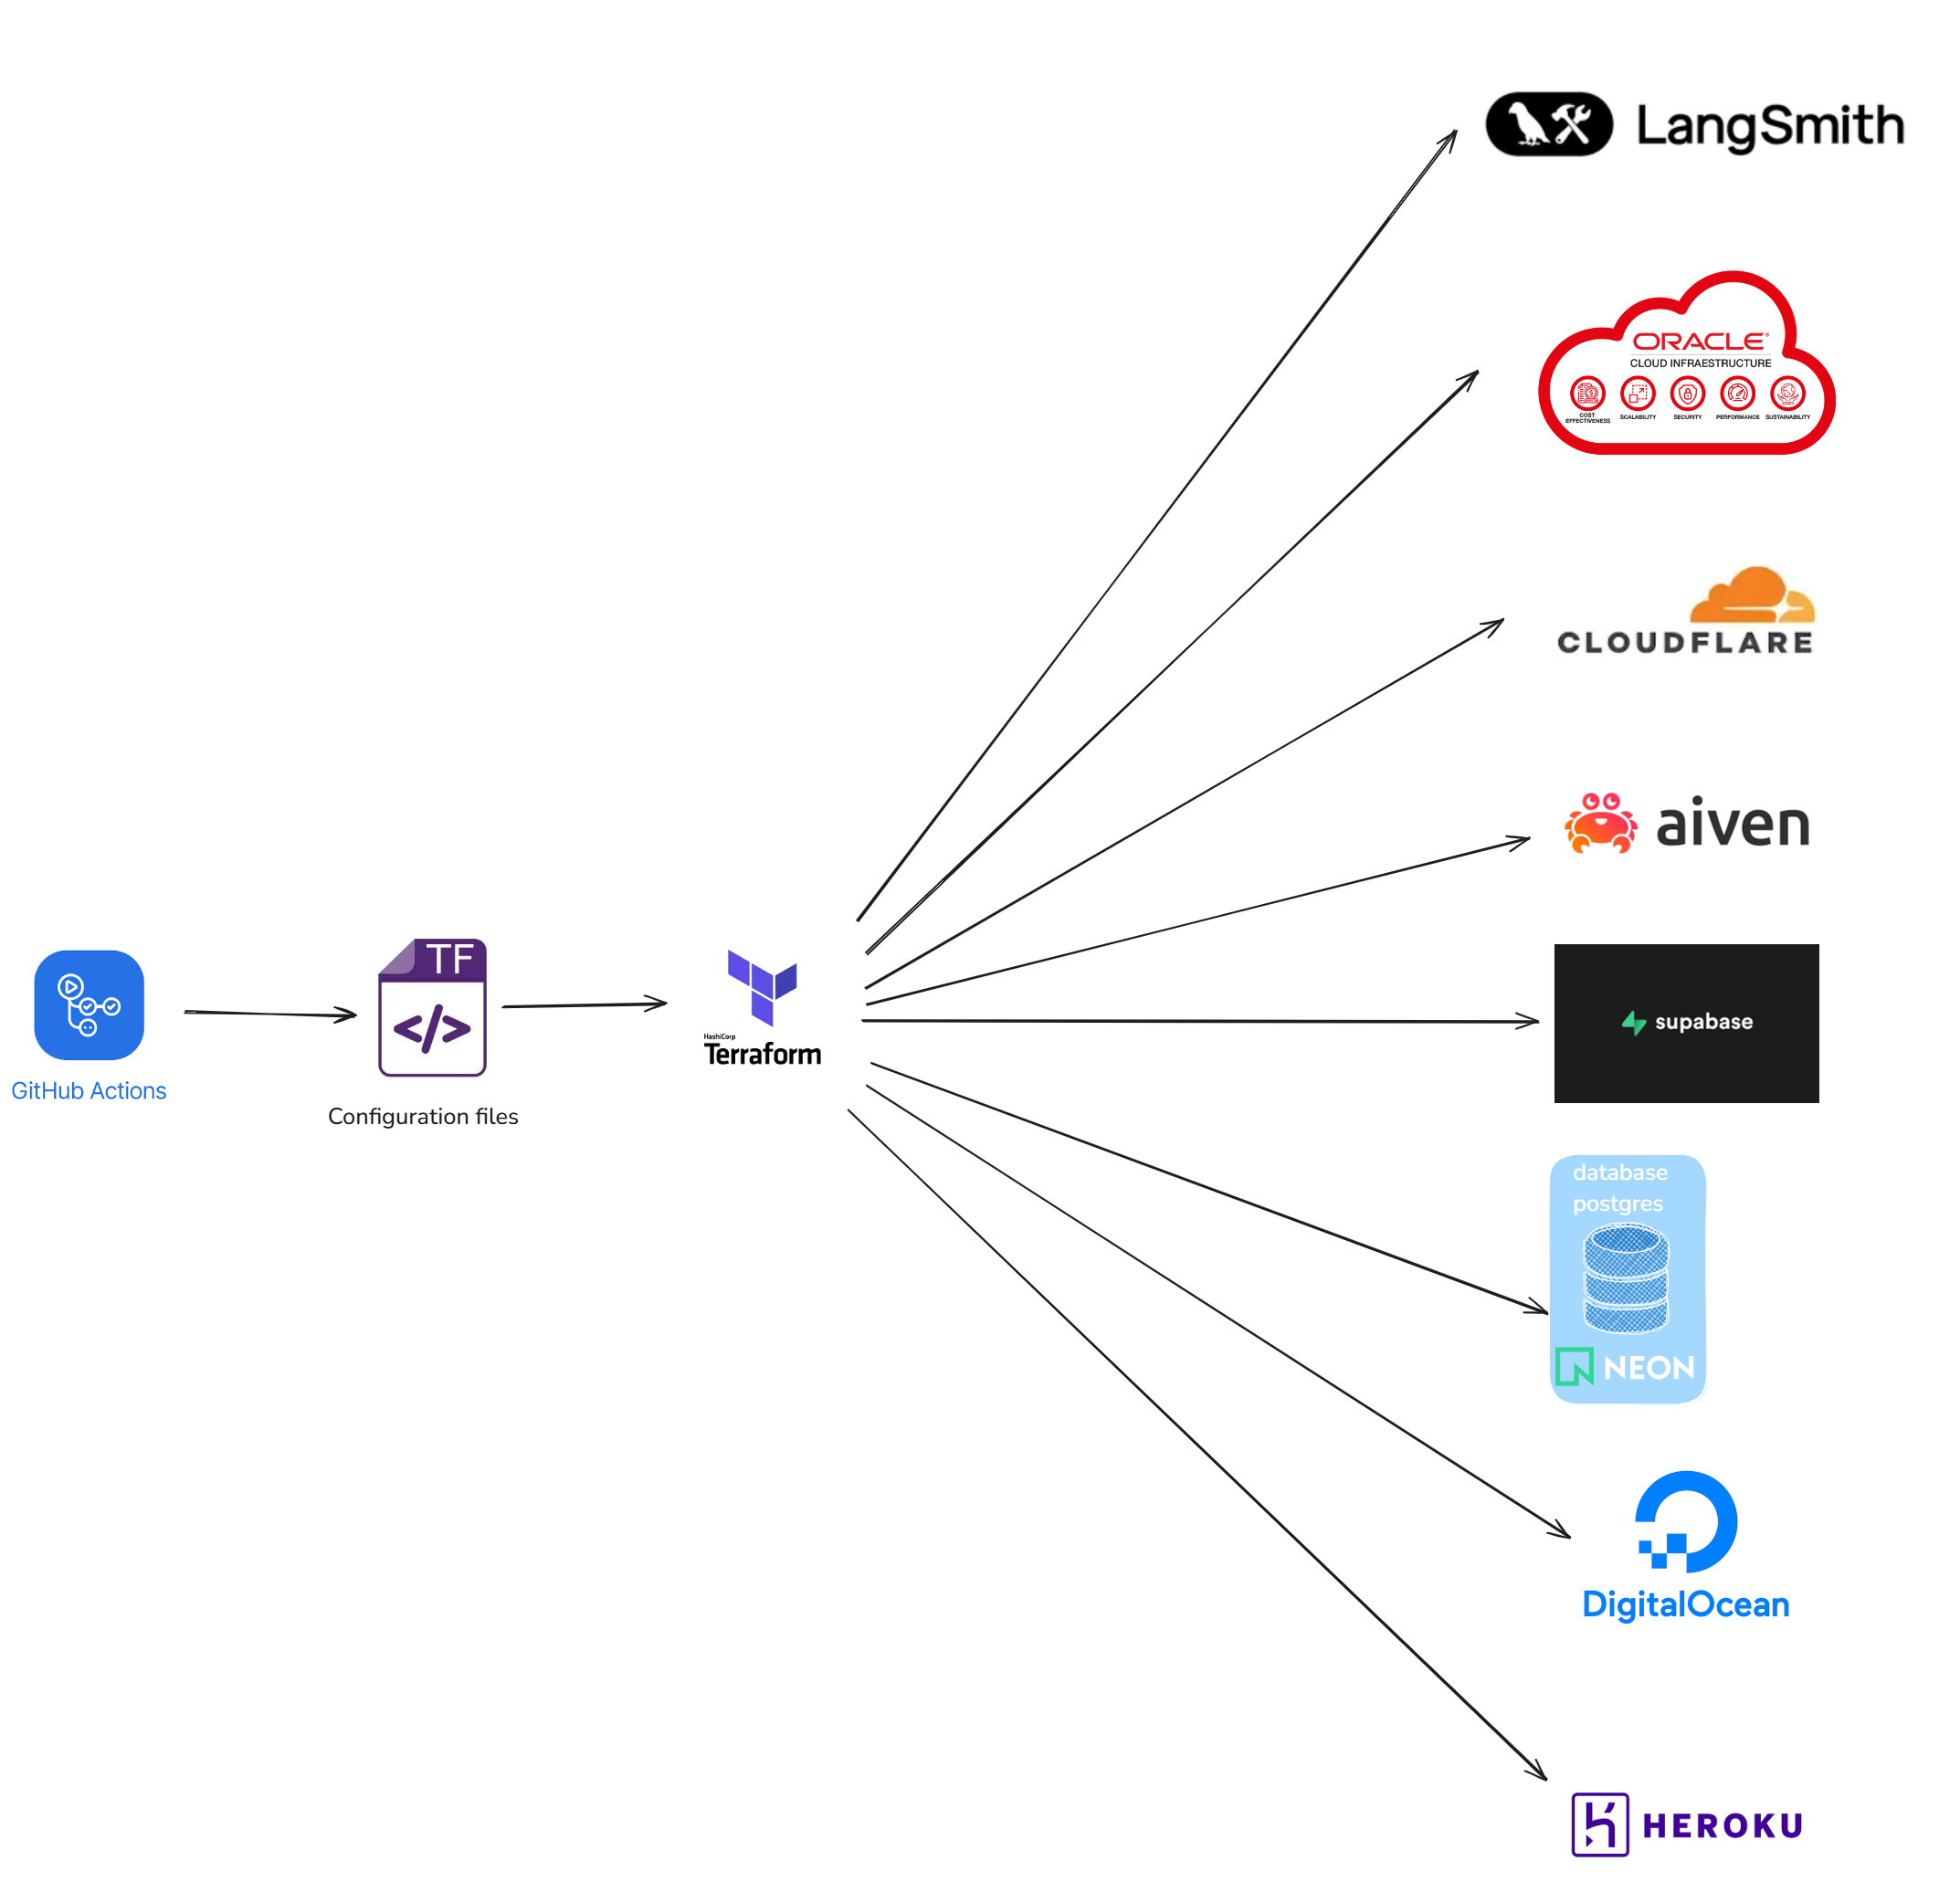
\includegraphics[scale = 0.2]{pictures/infrastructure-as-code-IaC-terraform.excalidraw.png}
\caption{Cấu hình chia nhỏ bí mật theo từng nhu cầu sử dụng trong doppler}
\end{figure}


Tại dự án
\url{https://github.com/20206205Tech/infra-by-terraform}
dùng root module lớn truyền biến
vào các module nằm trong thư mục modules.
Tuy nhiên việc chạy CI/CD có thể xảy ra lỗi vì provider bị lỗi,
hoặc mất thời gian chỉ vì thay đổi nhỏ cần terraform init
với nhiều provider không thay đổi.
Vì vậy, trong đồ án này,
em sử dụng mỗi provider trong folder riêng Tại dự án
\url{https://github.com/20206205Tech/infrastructure}.
Kết hợp github action chỉ chạy terraform khi có sự thay đổi của folder.

Cấu trúc dự án terraform với các folder riêng


\begin{figure}[H]
\centering
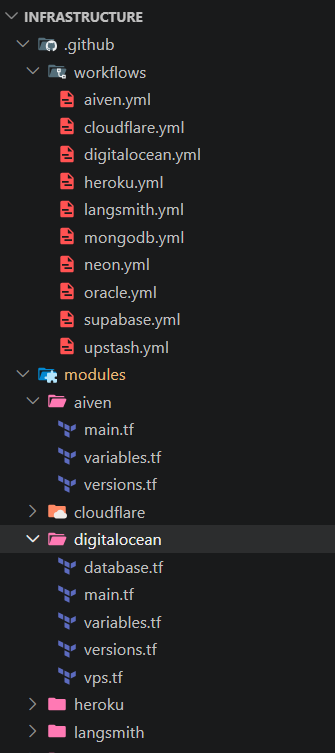
\includegraphics[scale = 0.2]{pictures/infrastructure-project.png}
\caption{Cấu hình chia nhỏ bí mật theo từng nhu cầu sử dụng trong doppler}
\end{figure}


Sử dụng Terraform Cloud để làm Remote Backend


\begin{figure}[H]
\centering
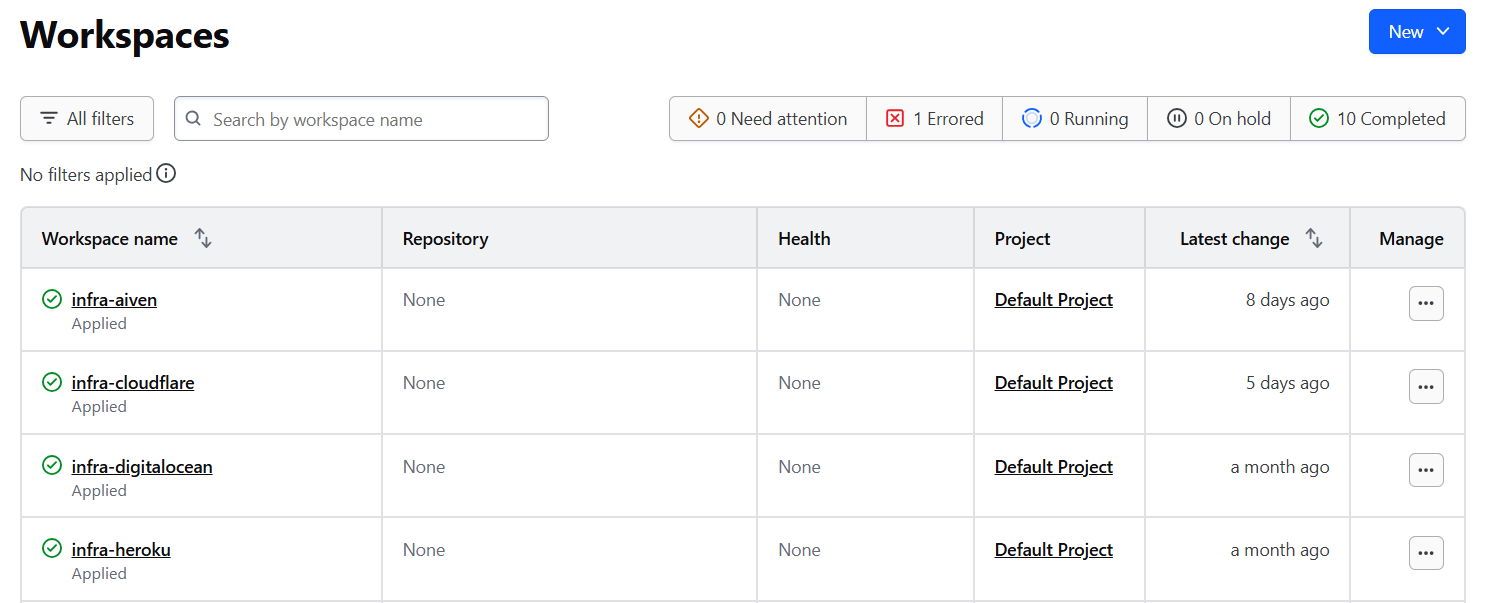
\includegraphics[scale = 0.2]{pictures/terraform-hub-web-ui.png}
\caption{Cấu hình chia nhỏ bí mật theo từng nhu cầu sử dụng trong doppler}
\end{figure}


\subsubsection{API Gateway trong Microservice (Kong API Gateway)}


API Gateway
được sử dụng
để quản lý và kiểm soát việc truy cập vào các API.
API Gateway cung cấp một lớp trung gian
giữa client và các microservices.
Có thể nói, API Gateway
là một điểm vào độc lập cho nhiều client của một ứng dụng.


Kong API Gateway
là một trong những API Gateway
mã nguồn mở
phổ biến
có thể quản lý các API được triển khai ở bất kỳ đâu, từ cơ sở hạ tầng đơn giản đến môi trường đa đám mây phức tạp.


\begin{figure}[H]
\centering
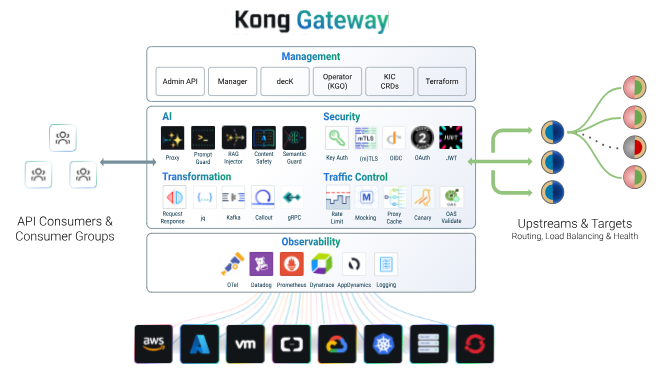
\includegraphics[scale = 0.2]{pictures/kong-gateway-overview.excalidraw.png}
\caption{Cấu hình chia nhỏ bí mật theo từng nhu cầu sử dụng trong doppler}
\end{figure}


Cấu trúc dự án Kong API Gateway


\begin{figure}[H]
\centering
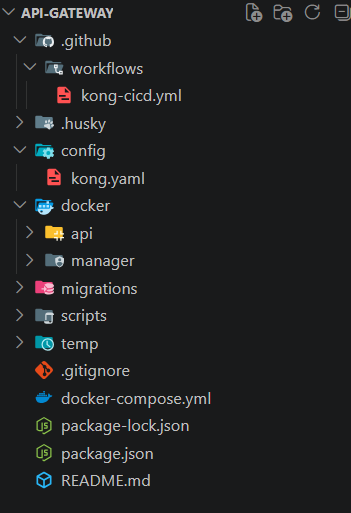
\includegraphics[scale = 0.2]{pictures/kong-api-gateway-project.png}
\caption{Cấu hình chia nhỏ bí mật theo từng nhu cầu sử dụng trong doppler}
\end{figure}


% TODO:

% Môi trường sản xuất thực tế gặp nhiều khó khăn, rate limmit giới hạn tốc độ
% DDOS
% dò env secret bí mật

% ![alt text](kong-api-gateway-env-secret.png)


\begin{figure}[H]
\centering
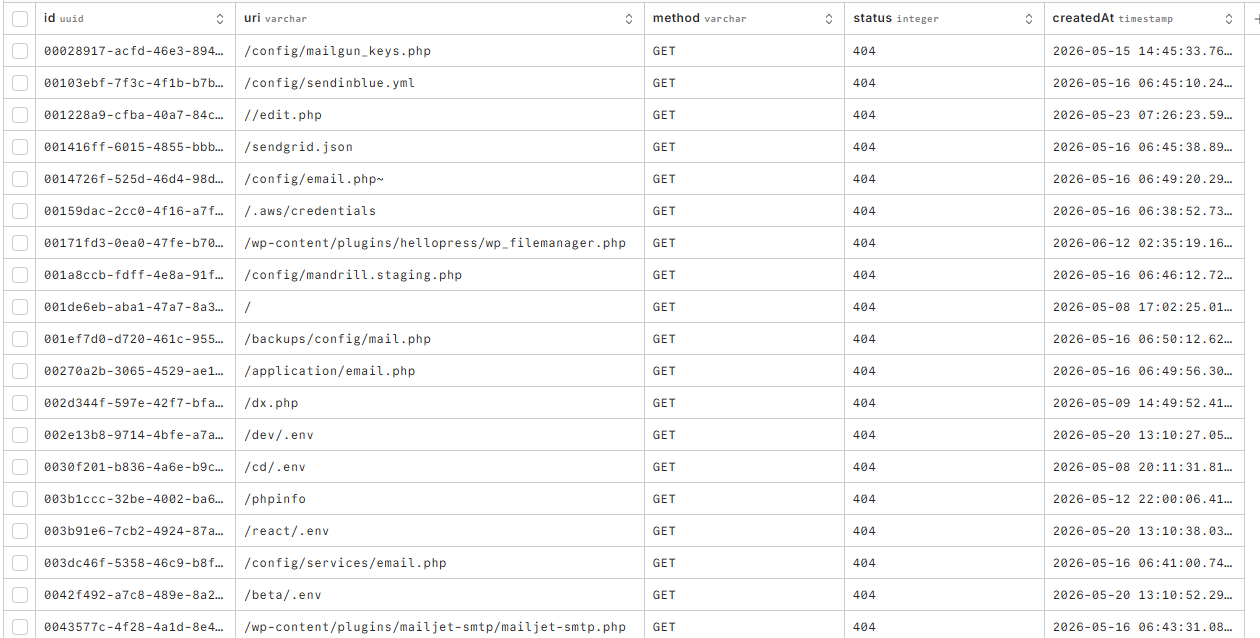
\includegraphics[scale = 0.2]{pictures/kong-api-gateway-env-secret.png}
\caption{Cấu hình chia nhỏ bí mật theo từng nhu cầu sử dụng trong doppler}
\end{figure}


Sơ đồ quản lý Kong API Gateway


\begin{figure}[H]
\centering
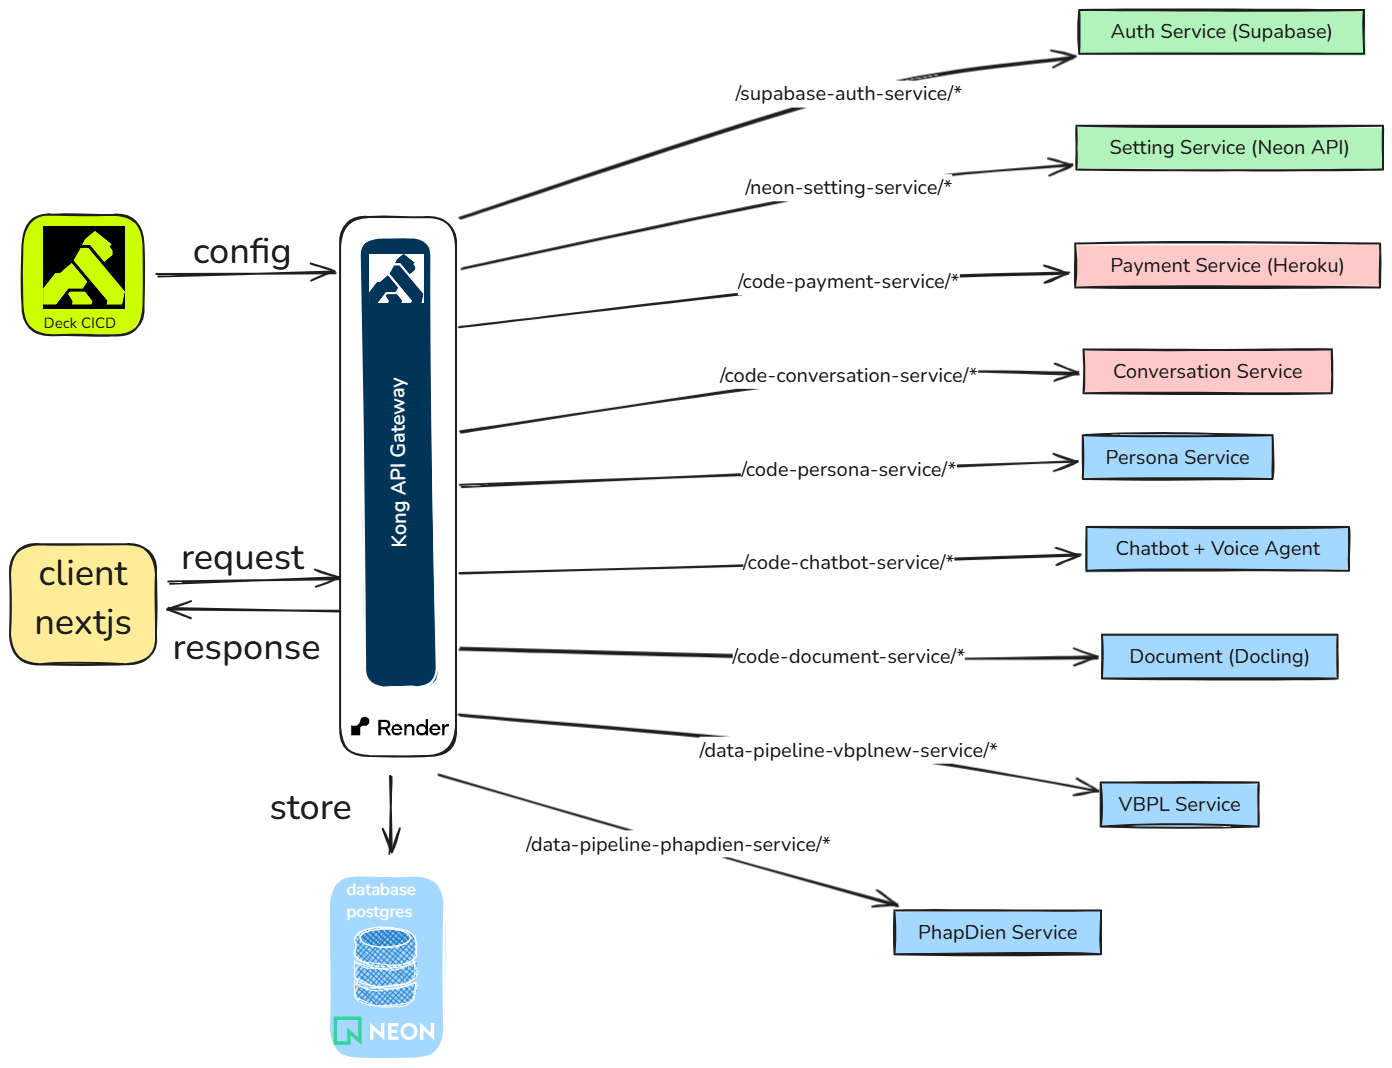
\includegraphics[scale = 0.2]{pictures/request-response-result-Kong-API-Gateway.excalidraw.png}
\caption{Cấu hình chia nhỏ bí mật theo từng nhu cầu sử dụng trong doppler}
\end{figure}


\begin{figure}[H]
\centering
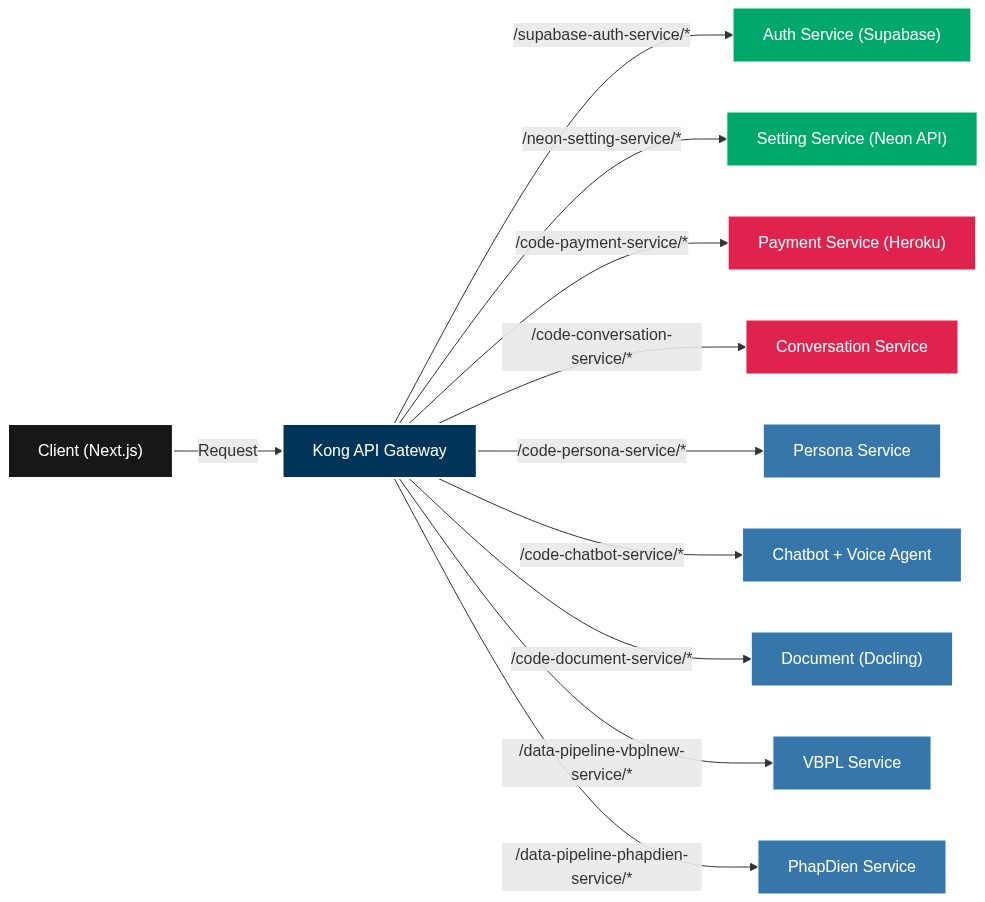
\includegraphics[scale = 0.2]{pictures/kong-api-gateway-router.png}
\caption{Cấu hình chia nhỏ bí mật theo từng nhu cầu sử dụng trong doppler}
\end{figure}

Có nhiều cách quản lý => ưu điểm của DECK


Các plugins trong dự án này:


\begin{itemize}
\item Plugin bot-detection: phân tích User-Agent và các dấu hiệu khác để chặn các request từ các bot độc hại, scraper, hoặc các công cụ tự động không mong muốn.

\item Plugin rate-limiting: giới hạn số lượng request, giúp bảo vệ các dịch vụ khỏi bị quá tải hoặc bị lạm dụng.

\item Plugin request-size-limiting: chặn các request có kích thước vượt quá ngưỡng cho phép.

\item Plugin http-log: thu thập các thông tin quan trọng về request/response và gửi qua giao thức http api NestJS và thực hiện lưu vào database postgres

\item Plugin correlation-id tạo request-id: tự động tạo ra một mã định danh duy nhất và gắn vào header của mỗi request để truy vết (tracing).

\item Plugin request-transformer thêm thông tin Request-Kong-Secret: gửi header chứa mã bí mật vào request trước khi đẩy xuống dịch vụ để các request phải được gọi từ Kong API Gateway.
\end{itemize}


\begin{figure}[H]
\centering
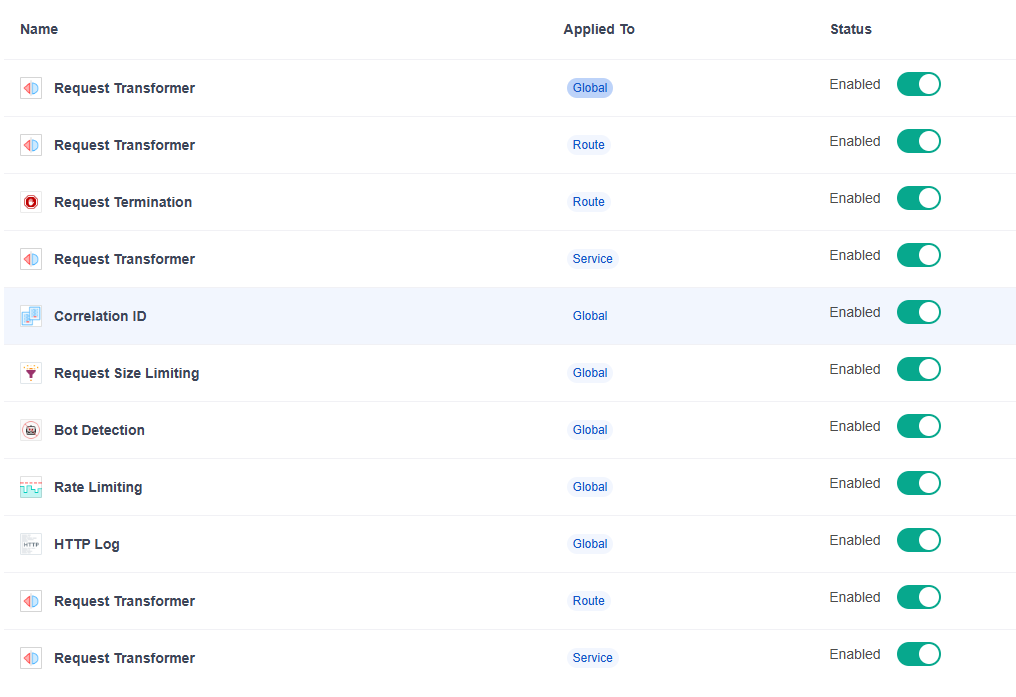
\includegraphics[scale = 0.2]{pictures/kong-api-gateway-plugin.png}
\caption{Cấu hình chia nhỏ bí mật theo từng nhu cầu sử dụng trong doppler}
\end{figure}
\begin{figure}[H]
\centering
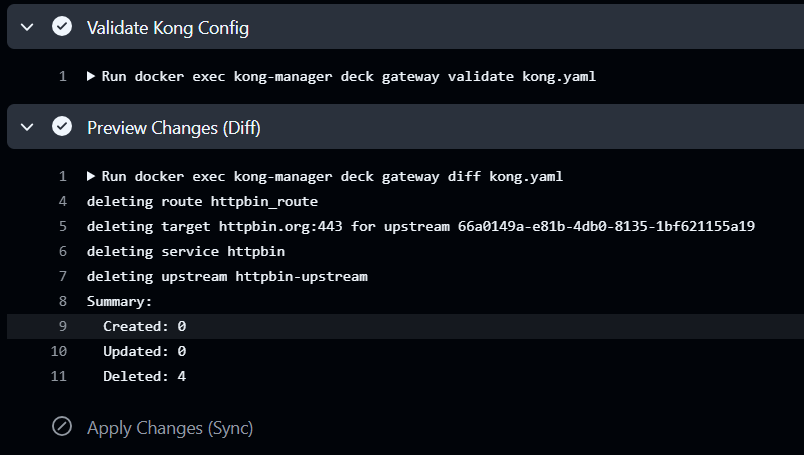
\includegraphics[scale = 0.2]{pictures/kong-api-gateway-github-action.png}
\caption{Cấu hình chia nhỏ bí mật theo từng nhu cầu sử dụng trong doppler}
\end{figure}
\begin{figure}[H]
\centering
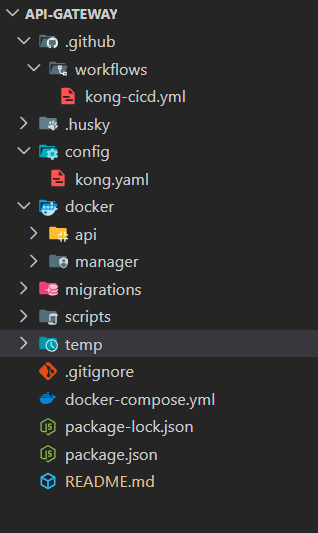
\includegraphics[scale = 0.2]{pictures/kong-api-gateway-folder.png}
\caption{Cấu hình chia nhỏ bí mật theo từng nhu cầu sử dụng trong doppler}
\end{figure}
